\subsection{Worksheet - Bead on a spinning circular wire}
\begin{center}
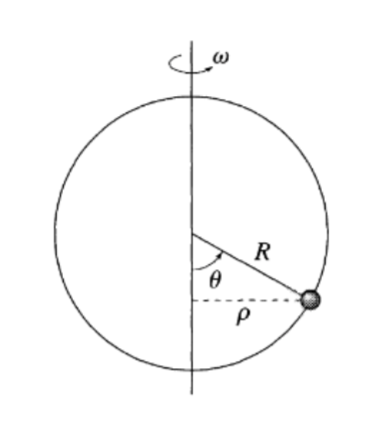
\includegraphics[scale=1]{Lecture-5/W5-img1.png}
\end{center}
A bead of mass $m$ is threaded on a frictionless circular wire hoop of radius $R$. The hoop lies in a vertical plane, which is forced to rotate about the hoop's vertical diameter with constant angular velocity $\dot{\phi} = \omega$. The bead's position on the hoop is specified by the angle $\theta$.

\begin{p}
Write an expression for the potential energy of the system.
\end{p}
\begin{s}
The height of the bead is determined (via trigonometry) to be $h = 1 - \cos\theta$, so the gravitational potential energy is given by:
\[U = mgh = mg(1-\cos\theta)\]
\end{s}

\begin{p}
Write an expression for the kinetic energy of the system. Thus you can now write out the Lagrangian $\LL$.
\end{p}
\begin{s}
\[T = \frac{1}{2}\frac{m}{v}\dot{\v{r}}^2 = \frac{m}{2}\left(R\omega\sin\theta + R\dot{\theta}\right)^2 = \frac{m}{2}\left(R^2\omega^2\sin^2\theta + R^2\dot{\theta}^2\right) \]
Where the first term is the normal velocity (out of the page in the diagram) and the second term is the tangential velocity (velocity in the frame of the page in the diagram). Hence the Lagrangian is:
\[\LL = T - U = \frac{m}{2}\left(R^2\omega^2\sin^2\theta + R^2\dot{\theta}^2\right) +mg(\cos\theta-1)\] 
\end{s}

\begin{p}
From the Lagrangian, what is the torque acting on the angle $\theta$ of the bead? What is the equation of motion for the bead?
\end{p}
\begin{s}
To get the torque, we look at the generalized force for $\theta$:
\[\dpd{\LL}{\theta} = -mgR\sin\theta + mR^2\omega^2\sin\theta\cos\theta\]
By the EL equation, we obtian the equation of motion for $\theta$:
\[ -mgR\sin\theta + mR^2\omega^2\sin\theta\cos\theta = \dod{}{t}\dpd{\LL}{\dot{\theta}} = mR^2\ddot{\theta}\]
\end{s}

\begin{p}
Sketch your best estimate for where the equilibrium point(s) of the bead are, i.e. sketch the equilibrium value(s) of $\theta_0$ versus $\omega$.
\end{p}
\begin{s}
There is an equilibrium point at the bottom of the ring (somewhat intuitively), and when the ring spins fast enough, there are additional equilibrium points symmetrically across the axis:
\begin{center}
    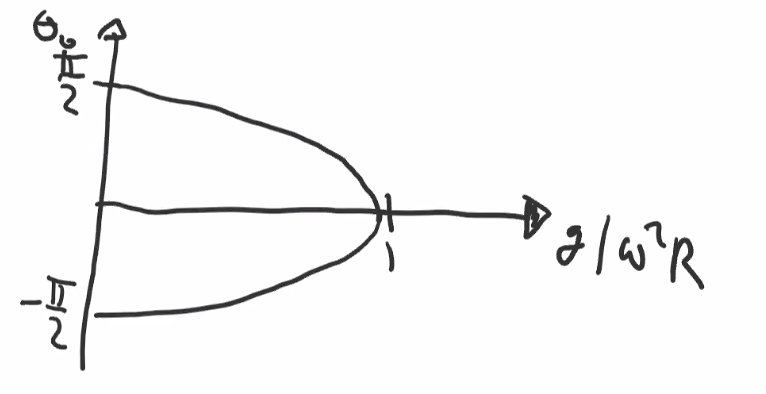
\includegraphics[scale=0.4]{Lecture-5/W5-img2.png}
\end{center}
The derivation of this graph and other equilibrium points mathematically is given in the next problem. We can see that as $\omega \rightarrow \infty$ that the bead will be perfectly horizontal (which lines up with our intuition somewhat).
\end{s}

\begin{p}
Convince yourself that an equilibrium point has $\dot{\theta} = \ddot{\theta} = 0$. Find all equilibrium points of the bead. Where is the equilibrium point when $0 < \omega^2 < g/R$?
\end{p}
\begin{s}
If we want equilibrium, we require the condition of $\ddot{\theta} = 0$ (as the bead should not feel any net torque and start with no angular velocity if it is to remain at rest), which results in \[\left(\omega^2\cos\theta_0 - \frac{g}{R}\right)\sin\theta_0 = 0\]
This has solutions of $\theta_0 = 0$ or $\theta_0 = \pi$ (the sine term is zero) or $\cos\theta_0 = \frac{g}{\omega^2R}$ or $\theta_0 = \pm \arccos(\frac{g}{\omega^2R})$. Since $\cos$ only varies between $1$ and $-1$ this arccos solution only has a solution for $\omega^2 \geq \frac{g}{R}$.
\end{s}

\begin{p}
Show that at the equilibrium points defined by $\omega^2\cos\theta - g/R = 0$, the tangential components of the gravitational and centrifugal forces (in the non-inertial frame of the hoop) cancel. Show that for any points with $\theta > \pi/2$ including near the top, the above two forces are in the same direction.
\end{p}
\begin{s}
Consider the balance of forces at these equilibrium points. There is the centrifugal force that throws the particle outwards, and the gravitational force that pulls the particle downwards. The centrifugal force is given by $\abs{\v{F}_{cent}} = m\omega^2r = m\omega^2R\sin\theta$ that throws the particle outwards and the gravitational force $\abs{\v{F}_g}= -mg$ downwards. We decompose these forces into the radial and tangential components.
\begin{center}
    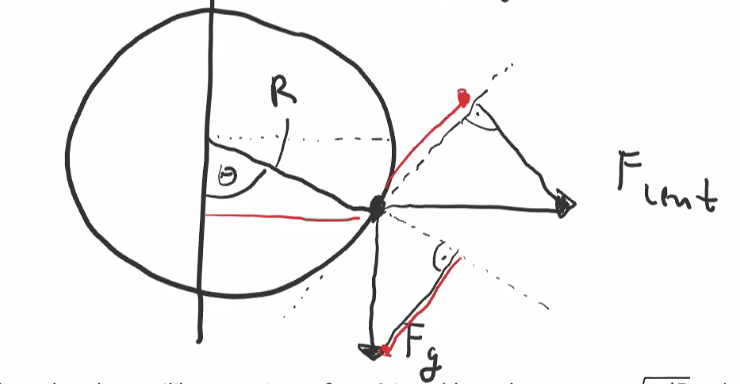
\includegraphics[scale=0.4]{Lecture-5/W5-img3.png}
\end{center}
For the angle to remain constant, we require that the tangential components (pictured in red above) must cancel. This is given by:
\[F_{tan} = -mg\sin\theta + m\omega^2R\sin\theta\cos\theta = \sin\theta\left(\omega^2 R\cos\theta - g\sin\theta\right)\]
Which we see is $0$ whenever $\omega^2\cos\theta - g/R = 0$ and hence we get the same answer in two different ways. 
If $\theta > \frac{\pi}{2}$, then we have that $\sin\theta > 0$ and $\cos\theta < 0$ and hence we can see from the above expression of the tangential force above that the gravitational tangent force and the centrifugal force point in the same direction; there is no hope of having an equilibrium point on the upper half of the metal loop!
\end{s}

\begin{p}
Show that the equilibrium point at $\theta_0 = 0$ is stable, so long as $\omega < \sqrt{g/R}$. What is the oscillation frequency about the equilibrium point?
\end{p}
\begin{s}
When $\theta$ is small, we can do a small angle approximation and so $\cos\theta \sim 1$ and $\sin\theta \sim \theta$. Going back to our equation of motion, we see that:
\[mR\ddot{\theta} = -mgR\theta + mR^2\omega^2\theta\]
and therefore:
\[\ddot{\theta} = \left(\omega^2 - \frac{g}{R}\right)\theta\]
Which is a nice equation we can solve analytically. We see that the RHS is negative when $\omega < \sqrt{\frac{g}{R}}$ and positive when $\omega > \sqrt{\frac{g}{R}}$. In the first case, the solutions to the differential equations are sines/cosines; i.e. simple harmonic oscillation with frequency $\Omega = \sqrt{\frac{g}{R} - \omega^2}$:
\[\ddot{\theta} = -\Omega^2\theta\]
\[\theta(t) = A\cos(\Omega t) + B\sin(\Omega t)\]
Which is a stable equilibrium; it oscillates about the $\theta = 0$ point when perturbed from it.
\end{s}

\begin{p}
Find the oscillation frequencies about the equilibrium points $\theta_0$ when $\omega > \sqrt{g/R}$. What is the stability condition for these oscillations? What is the oscillation frequency? Now sketch the equilibrium values of $\theta_0$, as a function of $\omega$, over the full range $\omega > 0$.
\end{p}
\begin{s}
Conversely, when $\omega > \sqrt{g/R}$, consider a small perturbation $\theta_0 + \e$ from the equilibrium. For a small $\e$, we have:
\[\cos(\theta_0 + \e) \approx \cos\theta_0 - \e\sin\theta_0\]
\[\sin(\theta_0 +\e) \approx \sin\theta_0 +\e\sin\theta_0\]
The equation of motion then becomes:
\[\ddot{\theta} = \left[\omega^2\cos(\theta_0 + \e) - \frac{g}{R}\right]\sin(\theta_0 + \e)\]
\[\ddot{\theta} \approx \left[\omega^2\cos\theta_0 - \e\omega^2\sin\theta_0 - \frac{g}{R}\right]\left[\sin\theta_0 + \e\cos\theta_0\right]\]
Now the $\omega^2\cos\theta_0$ and $-g/R$ terms cancel, and neglecting terms in $\e^2$, we have:
\[\ddot{\theta} = \ddot{\e} = -\e\omega^2\sin^2\theta_0 = -\Omega'\e\]
So we can see that if we perturb around $\theta_0$ that we have oscillation around $\theta_0$ which corresponds to a stable equilibrium. 
\end{s}
In conclusion, we see that this is quite a rich problem with respect to different equilibrium points and their behavior. There is also a discontinuous jump between certain equilibria $\omega = \sqrt{g/R}$, which is known as \textbf{bifurcation}, which can lead to chaotic motion.